\chapter{Fundamentação Teórica}\label{fundamentacao}
Nesta seção será apresentado os conceitos necessários para um completo entendimento deste trabalho. A \autoref{gerenciadeconfiguracao} conceitos inerentes a Gerência de configuração, juntamente com algumas ferramentas CASE e com ênfase em Integração Contínua descrito na \autoref{integracaocont} e por fim na \autoref{processonpi} será descrito o processo de gerência de configuração do NPI.

\section{Gerência de Configuração}\label{gerenciadeconfiguracao}
A gerência de configuração é a área da engenharia de software responsável pela evolução do software. Ela atua durante todo o ciclo de vida do produto de software e, por meio de técnicas, ferramentas e metodologias, visa garantir que as mudanças que irão ocorrer dentro do ciclo de vida do desenvolvimento do software sejam identificadas, avaliadas e comunicada a todos os envolvidos através de ferramentas que auxiliam neste processo de evolução.
Portanto "o propósito do processo de Gerência de Configuração é estabelecer e manter a integridade de todos os produtos de trabalho de um processo ou projeto e disponibilizá-la a todos os envolvidos"\space\cite{mpsbr}.
\subsection{Plano de Gerenciamento de Configuração}\label{pgc}
O Plano de Gerenciamento de Configuração (PGC) descreve todas as atividades de configuração e mudança que serão realizadas durante o projeto. Um conjunto de atividades, responsabilidades, ferramentas, recursos e etc. A gerência de configuração tem como objetivo garantir a integridade dos itens de configuração, que são qualquer artefato que esteja sob custódia da Gerência de Configuração, através do versionamento, da identificação, controlando mudanças e acesso. 

\subsection{Sistema de Controle de Versão}
Um sistema de controle de versão: "	[...] combina procedimentos e ferramentas para gerenciar diferentes versões de objetos de configurações que são criadas durante o processo de engenharia de software" \cite[p.~927]{pressman2010}.
Atualmente, o uso de sistema de controle de versão se tornou comum nas empresas de grande e pequeno porte. Tais ferramentas permitem que se tenha o controle de diferentes versões de arquivos que estão submetidos ao versionamento, recuperação de versões antigas, visualizar alterações realizadas em arquivos e saber por quem e quando o arquivo foi alterado. Através de comandos (i.e.,\textit{check-in},\textit{check-out}) os usuários conseguem se comunicar com o repositório a fim de obter os artefatos ali armazenados \cite{gleiph2011}. Em situações especais faz-se necessário que os desenvolvedores trabalhem em una linha diferente da original chamada de \textit{mainline}, geralmente essa situação ocorre quando tem-se como objetivo consertar bugs de versões anteriores do repositório, nesse caso um \textit{branch}, uma ramificação na linha de desenvolvimento do controle de versão, é criado afim de permitir a realização desta ação, permitindo assim o trabalho em paralelo sobre o mesmo repositório.
\begin{figure}[h]
\centering
\caption[Branch no Sistema de Controle de Versão]{Branch no Sistema de Controle de Versão.}
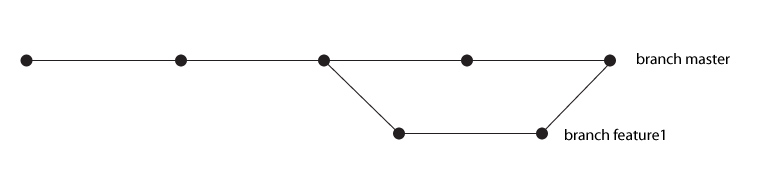
\includegraphics[width=0.5\linewidth]{./images/branch}
\label{fig:Branch}
\legend {\fontsize{10}{12}\selectfont {Fonte: \citeonline{tableless2012}}.}
\end{figure}
A figura \autoref{fig:Branch} demonstra a criação de um \textit{branch} paralelo a linha de desenvolvimento principal chamada de branch feature1 e branch master respectivamente, posteriormente as ações realizadas no \textit{branch feature1} são incorporadas ao \textit{branch master}.
\subsubsection{Sistema de Controle de Versão Local}
Um sistema de controle de versão local	armazenam todas as informações de um arquivo submetido ao versionamento na máquina local, guardando diferentes versões daquele arquivo localmente como demonstrado na figura \autoref{fig:SCVLocal}.
\begin{figure}[h]
\centering
\caption[Sistema de Controle de Versão Local]{Sistema de Controle de Versão Local.}
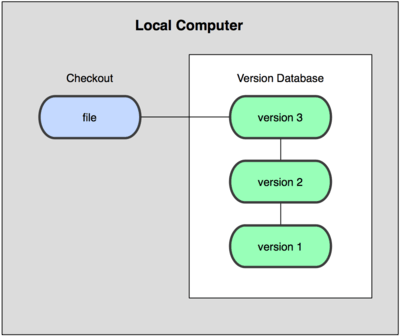
\includegraphics[width=0.5\linewidth]{./images/scvlocal}
\label{fig:SCVLocal}
\legend {\fontsize{10}{12}\selectfont {Fonte:\cite{git}}.}
\end{figure}
\subsubsection{Sistema de Controle de Versão Centralizado} Sistema de controle de versão centralizado como o nome diz possuem um único servidor centralizado, como o \textit{subversion} \footnote{http://subversion.apache.org}, \textit{perforce} \footnote{http://www.perforce.com}, este tipo de padrão de SCV mantém em seu único servidor todos os arquivos versionados. Para cada comando de comunicação realizado nos arquivos versionados, uma requisição deverá ser feita, podendo gerar lentidão ou deixar o servidor fora de funcionamento.
\begin{figure}[h]
\centering
\caption[Sistema de Controle de Versão Centralizado]{Sistema de Controle de Versão Centralizado.}
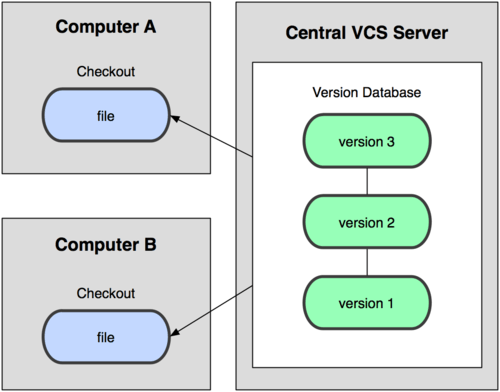
\includegraphics[width=0.5\linewidth]{./images/scvcentral}
\label{fig:SCVCentral}
\legend {\fontsize{10}{12}\selectfont {Fonte: \citeonline{git}}.}
\end{figure}
No exemplo acima dois desenvolvedores trabalhando em máquinas diferentes realizam a comunicação com o servidor central para obter o artefato de trabalho.	
\subsubsection{Sistema de Controle de Versão Distribuído}Os sistemas de controle de versão distribuído possuem um servidor central onde os arquivos são submetidos a versionamento, entretanto cada desenvolvedor possui em sua máquina de trabalho as versões que estavam no servidor, tornando cada \textit{workstation} um "servidor", portanto, caso ocorra um problema no servidor central, estes podem ser recuperados via \textit{workstation}, mantendo a integridade dos arquivos e evitando ser um ponto único de falha, como mostra a figura \autoref{fig:SCVDistribuido}.
\begin{figure}[h]
\centering
\caption[Sistema de Controle de Versão Distribuído]{Sistema de Controle de Versão Distribuído.}
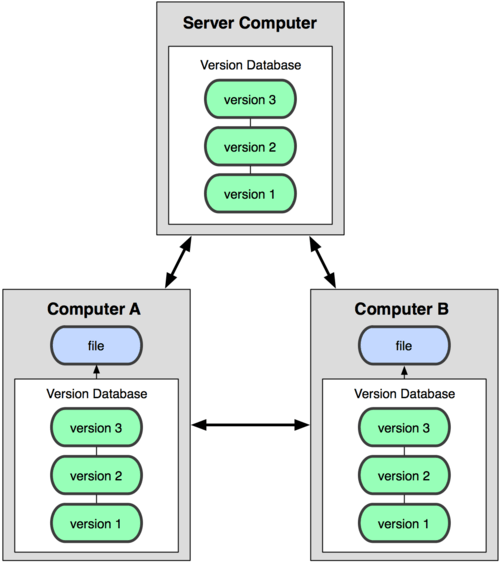
\includegraphics[scale=0.5]{./images/scvdist}
\label{fig:SCVDistribuido}
\legend {\fontsize{10}{12}\selectfont {Fonte: \citeonline{git}}.}
\end{figure}
\space

\subsection{Sistema de Controle de Mudança}
Todo software sofre mudanças, lidar com as mudanças é o papel da gerência de configuração, e para isso o gerente de configuração utiliza de um sistemas de controle de mudança. "O controle de mudança combina procedimentos humanos e ferramentas automatizadas para proporcionar um mecanismo de controle de mudança"\space \citeonline[p~.930]{pressman2010}. As mudanças devem ser avaliadas com cautela baseando-se, em seu custo benefício, uma combinação de esforço e \textit{business value}. A mudança tem início quando um "cliente" solicita a mudanças através de um formulário, conhecido como \textit{change request}. Nesse formulário é descrito os aspectos da mudança, após a solicitação ser realizada, esta deve ser avaliada, verificando se a mesma já foi solicitada, ou corrigida em caso de \textit{bugs}. Após a mudança ser validada, uma equipe de desenvolvedores avaliam os impactos que esta mudança têm sobre o sistema, verificando custo/benefício e esforço de realização \cite{sommerville2011}. Posterior a essa análise, a mudança será avaliada por um comitê de controle de mudança (CCB) que avaliará o impacto da perspectiva do negócio, o que decidirá se esta mudança será revisada, aprovada ou reprovada. Alguns sistemas que fornecem este controle sobre as mudança são: \textit{redmine \footnote{http://www.redmine.org}, GitHub \footnote{http://www.github.com} Jira \footnote{https://www.atlassian.com/software/jira}}
\subsection{Auditoria de Configuração}
"Uma auditoria de configuração de software complementa a revisão técnica formal ao avaliar um objeto de configuração quanto às características que geralmente não são consideradas durante a revisão"\space\citeonline[p~.934]{pressman2010}. Ela tem como objetivo garantir que mesmo com as mudanças realizadas a qualidade foi mantida. As auditorias se dividem em dois tipos: auditorias funcionais e auditorias físicas, a auditoria física baseia-se em verificar se os itens de configuração estão devidamente atualizados e se as práticas e padrões foram realizados da maneira correta, enquanto a auditoria funcional, busca verificar os aspectos lógicos dos itens de configuração.
\subsection{Ferramentas de Build}
As ferramentas de build tem como objetivo automatizar processos repetitivos, aumentando a produtividade e facilitando o trabalho do desenvolvedor. Através da definição de uma rotina, ou conjunto de comandos, o desenvolvedor informa a ferramenta que tipo de processo ele deseja automatizar, pode ser desde compilar e testar uma classe, como dropar e criar uma tabela nova no banco de dados, comprimir arquivos css e javascript, cabe ao desenvolvedor definir o escopo da automatização. Alguns exemplo deste tipo de ferramenta são: \textit{Ant, Grunt, Gulp, Maven}.


\begin{figure}[h]
\centering
\caption[Processo Lógico de uma Build]{Processo Lógico de uma Build.}
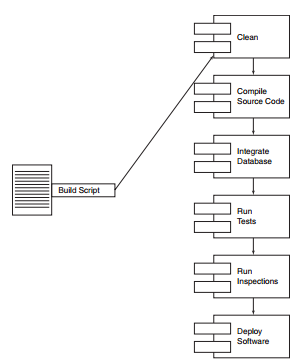
\includegraphics[scale=0.7]{./images/build}
\label{fig:build}
\legend {\fontsize{10}{12}\selectfont {Fonte: \citeonline{paul2007}}.}
\end{figure}
Na figura \autoref{fig:build} um script foi definido para realizar as seguintes funções, será realizado um clean no projeto, compilará o código fonte, integrará com o banco de dados, executará testes e inspeções no código e por fim será realizado o \textit{deploy} da aplicação.


%\subsection{Ferramentas de Integração Contínua}

\section{Integração Contínua}\label{integracaocont}
\begin{OnehalfSpace}
A integração contínua tem como objetivo identificar erros o mais rapidamente, permitindo que alterações efetuadas e integradas aos repositórios dos sistemas de controle de versão (SCV) sejam posteriormente verificadas e caso erros ocorram, estes sejam notificados imediatamente ao autor da alteração.
A melhor definição a cerca de integração contínua foi definida por \citeonline{fowler2000}
\end{OnehalfSpace}

\begin{citacao}
"[...] uma prática de desenvolvimento de software onde os membros de um time integram seu trabalho frequentemente, geralmente cada pessoa integra pelo menos diariamente – podendo haver múltiplas integrações por dia. Cada integração é verificada por uma build automatizada (incluindo testes) para detectar erros de integração o mais rápido possível. Muitos times acham que essa abordagem leva a uma significante redução nos problemas de integração e permite que um time desenvolva software coeso mais rapidamente." \citeonline[tradução nossa]{fowler2000}.
\end{citacao}

\subsection{Características de Integração}
Os requisitos para utilizar uma ferramenta de integração contínua de acordo com \citeonline{Anti2010} são:
\begin{itemize}
\item {\textbf{Uma conexão com um sistema de controle de versão:}}

A integração contínua necessita desta conexão, pois ela identifica as alterações ocorridas no repositório e dá início ao processo de integração.

\item {\textbf{A definição de uma build:}}

A integração contínua possui uma build privada que será executada assim que o processo de integração for iniciado, e é esta build que define que ações serão realizadas no processo de integração, tais como compilação, testes, análise de código.
\item {\textbf{Um mecanismo de feedback:}}

Um dos principais objetivos da integração contínua consiste em seu \textit{feedback} imediato, sendo assim um mecanismo deste tipo é essencial para a ferramenta, tais como e-mail, sms.
\item {\textbf{Um processo de integração do código: }}
O processo de integração consiste em como esta será realizada, manualmente ou através de um servidor de integração contínua de forma automatizada.

\end{itemize}

\subsection{Processo de Integração}
A integração ocorre quando alguma mudança é enviada ao sistema de controle de versão do repositório, que através de um servidor de integração contínua identifica a mudança e executa sua build privada \cite{mraz2013}. 


\begin{figure}[h]
\centering
\caption[Ambiente de Integração Contínua]{Ambiente de Integração Contínua.}
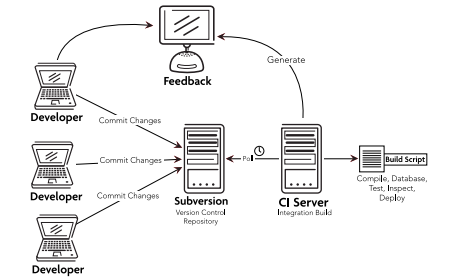
\includegraphics[scale=0.7]{./images/CI}
\label{fig:CI}
\legend {\fontsize{10}{12}\selectfont Fonte: \citeonline{paul2005}.}
\end{figure}

A \autoref{fig:CI} descreve um ambiente em que um servidor de integração contínua é utilizado. Existem três ambientes de trabalho distintos formado por três desenvolvedores que obtiveram uma cópia do projeto do repositório do SCV para trabalharem em suas \textit{workstation}, durante o trabalho alterações foram realizadas e commitadas ao repositório central, após a inserção junto ao repositório o servidor de integração contínua verifica as alterações e executa uma build de integração,  caso exista um problema com a build e esta não seja bem sucedida, o responsável pela alteração será informado sobre o ocorrido, assim seu objetivo em diante será a correção da build.

\subsection{Benefícios da Integração Contínua}

As principais vantagens em utilizar um servidor de integração contínua segundo \citeonline[p.~29]{paul2007} são:

\begin{itemize}
\item {\textbf{Redução de Riscos}}: 
Através da detecção imediada de código quebrados, ou incorretos, reduz-se risco atrelados ao produto.
\item {\textbf{Redução de processos manuais repetitivos}}:
Um conjunto de tarefas são executadas automaticamente pela build privada do servidor de integração contínua.
\item {\textbf{Permitir melhor visibilidade do projeto}}:
Através da identificação de informações inerentes ao desenvolvimento, como frequência de códigos defeituosos, módulos mais complexos, permitindo maior gerenciamento do projeto.
\item {\textbf{Estabelecer uma maior confiança no produto do time de desenvolvimento}}:
Através da visualizações de mudanças bem sucedidas, os desenvolvedores sentem maior confiança ao realizarem mudanças.
\end{itemize}

%\subsection{Integração Contínua e a Redução de Riscos}
%Os Riscos em produtos de software estão diretamente relacionados. Segundo \citeonline[p~.48]{paul2007} se você consegue reduzir certos riscos no software, você pode melhorar a qualidade do software.
\subsection{Builds Automatizadas}
Builds são rotinas de execução definidas com o objetivo de reduzir processos repetitivos. Durante o processo de desenvolvimento de um software muitas ações tendem a serem repetidas por parte dos desenvolvedores, utilizar o tempo para a realização  de atividades que poderiam ser automatizadas, de forma manual, reduz a produtividade e preocupações com melhorias devido ao tempo "apertado". Somando-se a isso, uma build garante que tudo que está nela definido será executado, evitando assim, que determinada ação seja esquecida, ou caso um novo membro entre na equipe uma explicação do que ele deve fazer, ou não esquecer de fazer, não faz-se necessário.

\subsection{Integração Contínua Manual}
Na IC manual o processo de integração é realizado individualmente, possibilitando que 
apenas um desenvolvedor realize check-in no repositório durante o intervalo de integração \citeonline{gleiph2011}. Este tipo de abordagem permite que apenas uma pessoa realize o \textit{check-in}, as integrações serão contínuas e seguidas, não paralelas. Este tipo de abordagem garante uma maior confiabilidade das integrações, pois segue um padrão de integração e os itens do repositório possuem maior consistência, e a garantia da estrutura do repositório é mantida \cite{gleiph2011}.

\subsection{Integração Contínua Automatizada}
A integração contínua automatizada é auxiliada pelo uso de um servidor de integração contínua, que obtém do controle de versão as alterações realizadas e executa sua build privada com o objetivo de verificar possíveis erros gerados por essas modificações.
\begin{citacao}
IC Automática possui a vantagem de ser escalável 
e,  deste  modo,  oferecer  maior  suporte  ao  trabalho  colaborativo.  Com  a  utilização  de 
Servidores  de  IC,  a  responsabilidade  de  realizar  construções  da  integração  é  retirada  dos desenvolvedores. Portanto, os desenvolvedores podem realizar  check-in  sem a necessidade de 
conquistar a vez de integrar. Esse fator é fundamental para que os  check-ins  continuem sendo 
verificados  sem  a  necessidade  de  um desenvolvedor  realizar  a  construção  e identificar 
problemas, resultando na eliminação do gargalo humano. \citeonline[p~.54]{gleiph2011}. 
\end{citacao}

\subsection{Processo de Escolha da Ferramenta}\label{escolhaFerramenta}
\begin{itemize}
\item {\textbf{Suporte a Linguagem:}}

O processo de escolha de um servidor de integração continua deve ser baseado de acordo com o suporte a linguagem, visto que alguns sistemas são construídos para trabalharem com uma linguagem de programação específica.

\item {\textbf{Suporte ao Sistema de Controle de Versão:}}

Como explanado anteriormente, a importância do SCV dentro de um servidor de integração contínua é altíssima, portanto escolher uma ferramenta que integre-se com o repositório é essencial, pois alguns servidor fornecem suporte a SCV mais populares, como \textit{Subversion}, \textit{Git}, entretanto pode não haver suporte ao \textit{Mercurial} por exemplo.


\item {\textbf{Segurança:}}

Garantir que somente pessoas autorizadas devem ter acessos aos artefatos existente no servidor de integração contínua.

\item {\textbf{Extensibilidade:}}

Capacidade dá ferramenta ter funcionalidades adicionadas por meio de \textit{plugins}, ser extensível.

\item {\textbf{Usabilidade:}}

Possuir baixa dificuldade na realização de ações dentro da ferramenta, boa aprendizagem, compreensibilidade.

\item {\textbf{Instalação e Configuração:}}

Facilidade de instalação em diferentes ambiente de operação, tais como sistemas operacionais, hardware através da utilização de recursos. Documentação clara e objetiva do processo de instalação.


\end{itemize}

\section{Processo do NPI}\label{processonpi}
O NPI possui um modelo de processo definido, este processo é baseado nos modelos e metodologias Scrum, MPS.BR e XP. Este modelo define as práticas e o modelo de trabalho dos envolvidos nas atividades do núcleo. Dentro do modelo de processo definido no NPI \footnote{http://www.npi.quixada.ufc.br/processo/} este trabalho tem como objetivo focar no modelo de processo de gerência de configuração.


\subsection{Processo de Gerência de Configuração do NPI}
O modelo de processo relacionado a gerência de configuração é descrito na figura \autoref{fig:procnpi}. Este modelo de processo possui duas atividade que serão descritas abaixo:
\begin{itemize}
\item \textbf{Criar Plano de Gerenciamento de Configuração:} Esta atividade é realizada pelo líder técnico da equipe envolvida. Esta atividade subdividi-se em quatro etapas são elas:
\begin{itemize}
\item \textbf{Identificar Itens de Configuração:} Esta atividade caracteriza-se pela criação, especificação e seleção dos produtos de trabalho, ferramentas, itens que tem objetivo descrever os produtos de trabalho. Exemplos de itens desta atividade são: Requisitos, Diagramas, Testes.

\item \textbf{Atribuir Identificadores únicos para os itens de configuração:} Esta atividade possui um nome bem sugestivo tem como intuito atribuir a cada item de configuração um identificador único de modo a facilitar a identificação dentro do projeto. O identificador segue o padrão $\left[PROJETO\right]$-$\left[TIPO\right]$-EXTRA.EXTENSÃO. Como exemplo um artefato possuiria o seguinte identificador: $\left[GPA\right]$-$\left[REQ\right]$-Especificacao.doc

\item \textbf{Identificar o responsável por cada item de configuração:} Esta atividade tem como objetivo atribuir a cada item de configuração um responsável, permitindo assim, uma maior facilidade na identificação do responsável de um determinado item de configuração.
\item \textbf{Criar	Plano de Gerenciamento de Configuração:} Esta atividade tem como objetivo a elaboração do PGC explicado na \autoref{pgc} por meio dos dados obtido com as tarefas anteriores. O plano define os responsáveis pelas atividades de Gerência de Configuração, ferramentas e ambientes a serem utilizados e todos os itens de configuração identificados.
\end{itemize}
\item \textbf{Estabelecer um sistema de Gestão de Configuração:} Esta atividade tem como requisito que o plano de gerenciamento de configuração esteja concluído, e possui apenas uma etapa:
\begin{itemize}
\item \textbf{Estabelecer um sistema de Gestão de Configuração:} Esta atividade tem como objetivo definir as ferramentas de acesso, ambiente de armazenamento e métodos para criação e alteração dos itens de configuração \cite{processonpi}. 
\end{itemize}
\end{itemize}

\begin{figure}[h]
\centering
\caption[Processo de Gerenciamento de Configuração]{Processo de Gerenciamento de Configuração.}
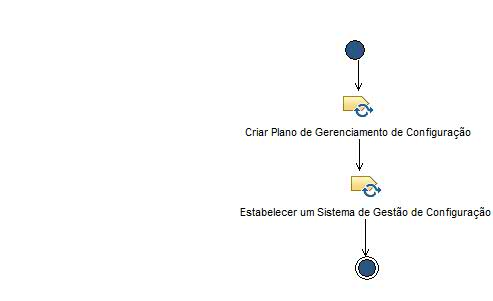
\includegraphics[scale=0.7]{./images/processonpi}
\label{fig:procnpi}
\legend {\fontsize{10}{12}\selectfont Fonte: \citeonline{processonpi}.}
\end{figure}

\section{Jenkins}
Jenkins, anteriormente conhecido como Hudson, é uma ferramenta de integração contínua \textit{open source}, que fornece suporte a projetos de diferentes linguagens e tecnologias ,.NET, Ruby, Grails, PHP, bem como Java, linguagem base de sua construção. \cite{smart2011}

\subsection{Jenkins no processo de escolha}\label{jenkinsEscolha}

\begin{itemize}
\item {\textbf{Suporte a Linguagem:}}

O jenkins permite suporte a uma grande gama de linguagens, tais como Java, PHP, Rails, Grails, Python, entre outras.

\item {\textbf{Suporte ao Sistema de Controle de Versão:}}
O Jenkins consegue realizar integrar nativamente com os principais sistemas de controle de versão tais como: \textit{CVS}, \textit{SVN},  \textit{Mercurial}, e \textit{Git} através da utilização de plugin.


\item {\textbf{Segurança:}}
A segurança do Jenkins é habilitada através de permissões e papéis, onde a base de dados de usuários pode ser pela base interna do Jenkins, LDAP, usuários do sistema operacional e também através do usuário vinculado ao GitHub.

\item {\textbf{Extensibilidade:}}
Jenkins é extremamente flexível e adaptável, permitindo assim oferecer uma melhor atuação para diferentes propósitos, através das centenas de plugins disponíveis. Plugins este que oferecem tudo desde sistemas de controle de versão, ferramentas de build, ferramentas de análise estática de código, notificadores de build, alterações de UI, integração com sistemas externos (\textit{Jira, Redmine}) \cite{smart2011}.


\item {\textbf{Usabilidade:}}
"Primeiramente, Jenkins é fácil de usar. A interface é simples e intuitiva, e o Jenkins como um todo possui uma curva de aprendizado baixa" \citeonline[p~.3]{smart2011}.

\item {\textbf{Instalação e Configuração:}}

Facilidade de instalação, diferentes ambiente de operação, tais como sistemas operacionais, utilização de recursos. Documentação clara e objetiva do processo de instalação informando dependência existentes.


\end{itemize}
